\section{Rendering und Physik}

\subsection{Objekte}
	Die Szene lässt sich einteilen in Billiard-Pool und Billiard-Kugeln.
	Der Pool besteht aus einer grünen Fläche und 6 Löchern.
	Er besitzt zudem ein 2:1 Verhältnis von Breite zu Höhe. \\
	
	Die Grüne Farbe ist lediglich die Clear-Color unseres OpenGL Kontextes. 
	Dies können wir machen, weil es sich um eine 2D Anwendung handelt und niemals etwas über den Boden hinaus gezeichnet werden muss. 
	Die Löcher werden simuliert, indem ein sogenannter Triangle-Fan gebaut wird.\\
	
	Im Folgenden gehen wir zur Vereinfachung davon aus, dass wir stets nur 2 Koordinaten haben, da die z-Koordinate aufgrund der Zweidimensionalität der Anwendung immer 0 ist. \\
	
	Die Struktur beginnt in der Mitte beim zum Objekt Relativen Punkt $(0,0)$.
	Von dort aus werden Dreiecke aufgespannt. 
	Wir benötigen immer nur die  Koordinaten von dem Randpunkt, der im Uhrzeigersinn weiter verschoben ist, da der GL-Triangle-Fan immer den neuen Punkt mit dem letzten Randpunkt und dem Mittelpunkt verbindet. 
	Der darauf folgende Punkt wird berechnet durch die Anzahl der Punkte die wir haben wollen, hier genannt $k$ und der Berechnung von Kreis-Koordinaten: \\
	
	$\delta$ ist der Grad, um den in jedem Schritt der Punkt auf dem Umriss verschoben wird. 
	Dabei muss gelten $\delta \cdot k = 360$ damit wir einen ganzen Kreis bekommen.\\
	
	\begin{equation}\label{eq:delta}
		\delta =\frac{2 \cdot \pi}{k} 
	\end{equation}
	Sei n der gewünschte Radius von der Kugel und i der aktuelle Schritt in der Schleife von $i=1$ bis k, dann sind die Koordinaten für die Punkte auf dem Kreis:
	\begin{equation}\label{eq:circleCoord}
		\begin{aligned}
			x = \cos (\delta \cdot i) \cdot n\\
			y = \sin (\delta \cdot i) \cdot n
		\end{aligned}
	\end{equation}
	Wenn wir nun $k$ mal die Koordinaten berechnet haben haben wir einen fertigen Kreis, bestehend aus $k$ Dreiecken. Diese werden nun an den 4 Ecken des Spielfeldes angebracht, sowie bei $(w /2 h)$ und $(w/2, 0)$, mit $w$ = Breite des Spielfeldes in Pixeln, $h$ = Höhe des Spielfeldes in Pixeln. \\
		\begin{figure}[h]
		\centering
		\caption{Vollständiger Triangle-Fan mit k=12}
		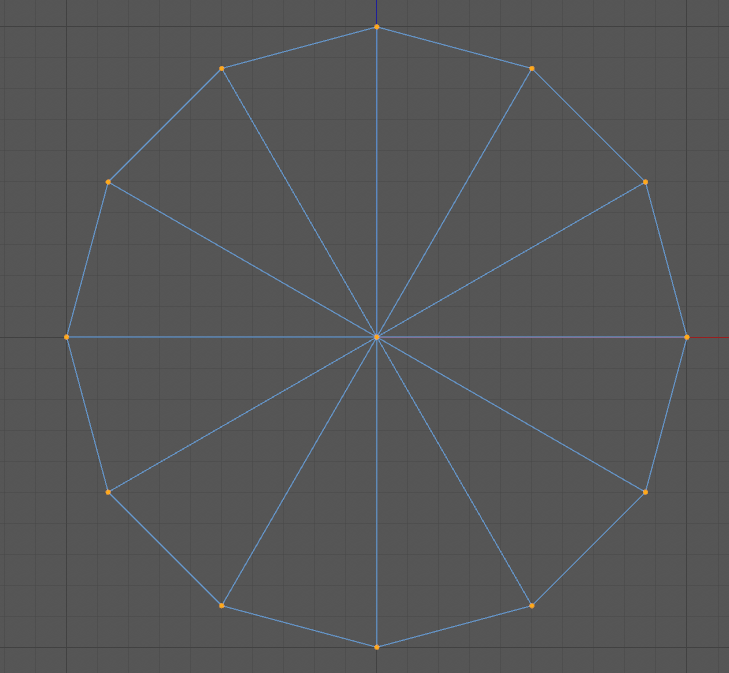
\includegraphics[width=\textwidth/2]{bilder/k12kreis.png} \\
	\end{figure} \\
	Man sieht, dass wenn man nur $k = 12 $ benutzt, ist der Kreis nicht rund genug. Deshalb sollte man einen Wert nehmen der für die Ansprüche genügt. Wir haben uns aufgrund der Größe unserer Kreise für $k=64$ entschieden um die beste Rundung zu erhalten.\\
	Diese Form der Kreisberechnung können wir auch für die Billiard-Kugeln anwenden.
	\begin{figure}[h]
		\caption{Spielfeld ohne Texturen}
			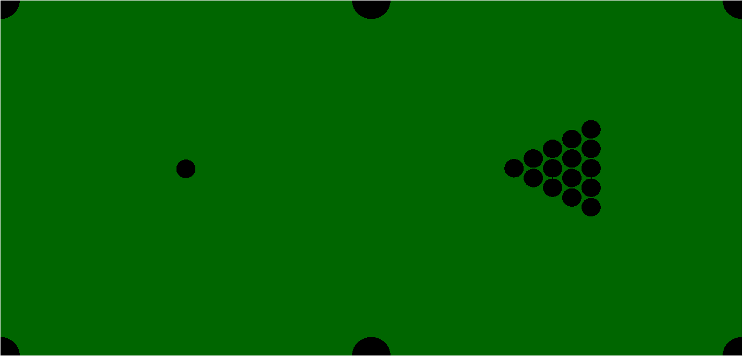
\includegraphics[width=\textwidth]{bilder/untextured_pool_low.png} 
	\end{figure}

\subsection{Texturierung}
	Die Farben für das Spielfeld sind trivial. 
	Die Kugeln hingegen müssen vom Spieler unterschieden werden können. 
	Wir müssen also Texturen auf Kreise abbilden. 
	Dazu haben wir zunächst eine Textur erstellt: \\
	\begin{figure}[h]
		\caption{Billiardkugel Textur}
			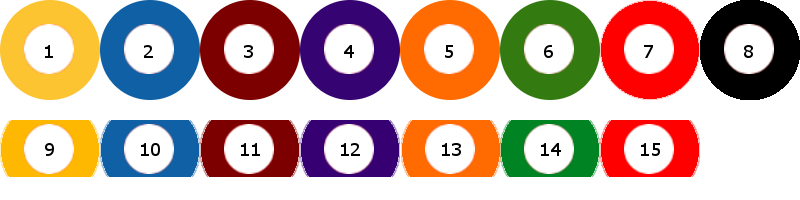
\includegraphics[width=\textwidth]{bilder/Balls.png} \\
	\end{figure} \\
	Nun müssen wir die Textur auf einen Kreis bekommen. 
	Dazu verwenden wir u/v-Koordinaten. 
	Unsere Textur besitzt auf beiden Achsen einen Wertebereich von 0 bis 1. 
	Dabei ist $(0,0)$  oben links und $(1,1)$  unten rechts. 
	Da wir die Texturen für alle Kugeln in einer Datei gespeichert haben, können wir jetzt anhand der u/v-Koordinaten der Textur jeder Kugel einen Ausschnitt zuweisen.
	Dafür werden den Farben der Kugeln werte nach ihrer Reihenfolge auf der Textur gegeben: 
	\begin{equation}\label{eq:color}
	c = 
	\begin{cases}
		0, & \text{falls Gelb} \\
		1, & \text{falls Blau} \\
		2, & \text{falls Rot} \\
		3, & \text{falls Lila} \\
		4, & \text{falls Orange} \\
		5, & \text{falls Grün} \\
		6, & \text{falls Rot} \\
		7, & \text{falls Schwarz oder Weiß}
	\end{cases}
	\end{equation} 
	Außerdem bekommt jede Kugel gesagt, ob sie Halb oder Voll ist, wobei Voll = 0 ist und Halb = 1.  \\
	\begin{equation} \label{eq:full}
	f = 
	\begin{cases}
		0, & \text{falls Kugel voll} \\
		1, & \text{falls Kugel halb}	
	\end{cases}
	\end{equation}\\
	\begin{figure}[h]
		\caption{Textur mit u/v-Koordinaten}
		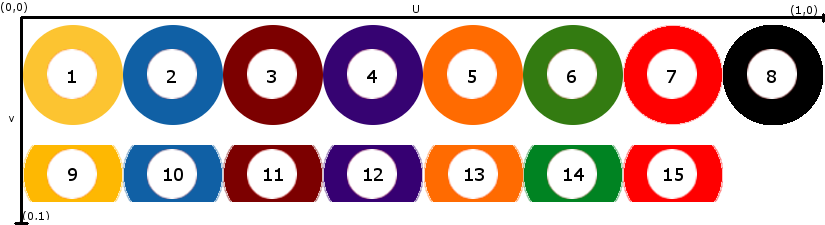
\includegraphics[width=\textwidth]{bilder/ballsachsen}
	\end{figure} \\
	Nun können wir uns eine Funktion erstellen, die anhand von Farbe und Fülle die Textur ausschneidet und auf die Kugel abbildet. 
	Dazu berechnen wir zuallererst die Anfangsposition der Textur. 
	Diese setzt sich zusammen aus der Farbe c und der Fülle f. \\
	Vorgedanke: Der Durchmesser einer Kugel auf unserer Textur ist $\frac{1}{8}$ für x, weil es 8 Kugeln pro Reihe gibt und die u Koordinate genau 1 lang ist, aber $\frac{1}{2}$ für $y$, weil es nur 2 Reihen gibt und die Textur trotzdem auf der v Achse 1 lang ist. 
	Somit liegt der Mittelpunkt der gelben vollen Kugel $(\frac{1}{16}, \frac{1}{4})$, weil dieser bei genau einer Halben Kugel Distanz auf beiden Achsen liegt. \\
	Kommen wir nun zur tatsächlichen Berechnung der Textur-Koordinaten: \\
	Mittelpunkt m der Textur: \\
	\begin{equation}\label{eq:texStart}
	\begin{aligned} 
		x = \frac{1}{16} + \frac{1}{8} \cdot c, c = \text{Farbe der Kugel \eqref{eq:color}} \\
		y = \frac{1}{4} + \frac{1}{2} \cdot f, f = \text{Fülle der Kugel \eqref{eq:full}}
	\end{aligned}
	\end{equation}
	Nun fehlen noch die Texturkoordinaten für den Kreis um den Mittelpunkt der Textur herum analog zum erstellen der Kreise mit dem Triangle-Fan. Die Berechnung läuft dabei genau wie die, der Koordinaten des eigentlichen Kreises, mit dem Unterschied in der Skalierung und Startposition. 
	So benutzen wir nicht den Radius der Kugeln des Spiels, sondern die Größe der Kugel auf der Textur und als Startpunkt haben wir nicht immer $(0,0)$ sondern unser vorher berechnetes x und y in \eqref{eq:texStart}. 
	\begin{equation}\label{eq:texXY}
	\begin{aligned}
		 xTex =  x + \cos(\delta \cdot i) \cdot \frac{1}{16}, \\
		 yTex =  y + \sin(\delta \cdot i) \cdot \frac{1}{4}, \\
		\text{mit } \delta \text{ nach }\eqref{eq:delta} \text{ und } i \text{ nach } \eqref{eq:circleCoord}
	\end{aligned}
	\end{equation}
	Die Textur wird dann beim erstellen des Triangle-Fans auf die Dreiecke gezeichnet. Dabei bekommen die Dreiecke für den Startknoten $(0,0)$ immer $(x,y)$ als Texturkoordinaten (\eqref{eq:texStart}) und der Randpunkt bekommt dann $(xTex,yTex)$ (\eqref{eq:texXY}.
\subsection{Kollisionsberechnung}
	Die Kollisionsberechnung lässt sich aufteilen in 3 Bereiche: \begin{itemize}
		\item [1.] Kollision von Kugeln mit Wand und Löchern
		\item [2.] Kollision von Kugeln mit anderen Kugeln
		\item [3.] Kollision der Weißen Kugel mit dem Queue
	\end{itemize}
	\subsubsection{Kollision von Kugeln mit Wand und Löchern}
		Das Kollidieren mit den Wänden ist sehr simpel: Wir geben  unsere Breite und Höhe des Spielfeldes als Grenzen an. Wenn die Kugel zu nah an eine der Wände kommt wird ihre Geschwindigkeit umgekehrt. Dementsprechend machen wir eine Fallunterscheidung mit 4 Fällen für die 4 verschiedenen Wände: \begin{itemize}
			\item [1.] Die Linke Wand (x=0)
			\item [2.] Die Rechte Wand (x=w)
			\item [3.] Die Obere Wand (y=0)
			\item [4.] Die untere Wand (y=h)
		\end{itemize}
		Dabei gilt wieder $ h = $ Höhe des Spielfeldes und $ w = $ Breite des Spielfeldes. \\
		Wenn nun einer der Fälle eintritt, wird die Geschwindigkeit auf der Achse, die getroffen wurde, invertiert. Beispiel: Die Kugel stößt an die linke Wand (x=0). Dann hat diese vorher eine negative Geschwindigkeit auf der x-Achse, weil sie Richtung x=0 sich bewegt hat. Wenn wir diese Geschwindigkeit nun umkehren, rollt die Kugel Richtung +x und somit wieder Weg von der Wand. So simulieren wir die Kollision. \\
		Nun kommen die Löcher als Einschränkung hinzu: Damit die Kugeln in die Löcher fallen können, müssen wir Lücken in den Wänden erzeugen. 
		Diese simulieren wir durch weitere Bedingungen. Jeder der 4 vorherigen Fälle, bekommt nun eine  Einschränkung. 
		Die Kugeln müssen einmal an allen Ecken, und dann bei $x= \frac{w}{2}\land (y= 0 \lor y = h)$ durch die Wand können. 
		Dass heißt wir überprüfen bei den x-Achsen Kollisionen ( $x=0$ und $x=w$ ), ob wir auf der y-Achse zwischen beiden Löchern sind und nicht am Rand. 
		Das lässt sich darstellen als: 
		\begin{equation}
		vy = \begin{cases}
			-vy, & \text{ falls } y \leq (h- l) \land y \geq l, \text{ mit } l = \text{größe der Löcher} \\
			vy, & sonst 
		\end{cases}
		\end{equation}
		Das gilt für Fall 1 und 2. Für Fall 3 und 4 benötigen wir noch eine Bedingung mehr:
		 \begin{equation}
		vx = \begin{cases}
		-vx, & \text{ falls } (x \leq (w/2 - l) \land x \geq l) \lor (x \geq (w/2 + l) \land (x \leq (w- l) \\
		vx, & sonst 
		\end{cases}
		\end{equation}
		Wir überprüfen also, ob die Kugel eine der Beiden Strecken zwischen den Löchern trifft, wenn sie vorher den Rand des Spielfeldes erreicht hat. 
	\subsubsection{Kollision mit anderen Kugeln}
		Für die Kollision zwischen den Kugeln müssen wir in jedem Frame berechnen, wie sich jede Kugel zu jeder anderen verhält und wenn sich diese treffen, in welche Richtung sie weiter Rollen. Dazu schauen wir uns immer nur 2 Kugeln an, wobei immer nur die erste verändert wird. 
		Die Kollisionsberechnung war uns bereits vorgegeben aus einem Beispiel für ein AirHockey Spiel. 
		Der Unterschied liegt darin, dass im Airhockey nur eine Kugel aktiv ist und diese mit zwei nicht von der Kollision betroffenen Schlägern kollidiert. 
		Somit haben wir, statt zu testen, ob die Kugel mit einem der beiden Schläger zusammenstößt, die Kollision von jeder Kugel mit allen Anderen berechnet. Dadurch müssen wir die Kollisionsmethode nicht abändern.
		Damit wird in jedem Frame überprüft, ob eine Kugel mit einer anderen Kollidiert und das für alle Kombinationsmöglichkeiten von 2 Kugeln. 
		Dabei muss natürlich darauf geachtet werden, dass keine Kugel mit sich selbst kollidiert. \\
		
		%\begin{equation}
		%d = \sqrt{(x_2 - x_1)^2 + (y_2-y_1)^2} 
		%\end{equation}
		%Wenn diese Distanz kleiner ist als der Durchmesser $r*2$ einer Kugel, dann gibt es eine Kollision. \\
%		Die Kollision wird ausgewertet, indem zunächst die Normale berechnet wird: 
%		\begin{equation}
%		\begin{aligned}
%		nx = x_1 - x_2; \\
%		ny = y_1 - y_2; \\
%		\end{aligned}
%		\end{equation}
%		Das Ergebnis $(nx,ny)$  wird dann noch normalisiert. Dann berechnen wir die Tangente dazu:
%		\begin{equation}
%		\begin{aligned}
%		tx = -ny \\
%		ty = nx
%		\end{aligned}
%		\end{equation}
%		Als nächstes wird die Relative Geschwindigkeit zwischen beiden Kugeln berechnet. Dabei bezeichnen wir die Geschwindigkeit einer Kugel als vx bzw. vy (also $vx_1$ für die Geschwindigkeit auf der X-Achse der Kugel $b_1$).
%		\begin{equation}
%		\begin{aligned}
%		vrx = vx_2 - vx_1 \\
%		vry = vy_2 - vy_1
%		\end{aligned}
%		\end{equation}

	\subsubsection{Zusammenfassung}
		 Nun haben wir ein Spielfeld mit Texturierten Kugeln die miteinander kollidieren.
		 \begin{figure}[h]
		 	\caption{Fertiges Spielfeld}
		 	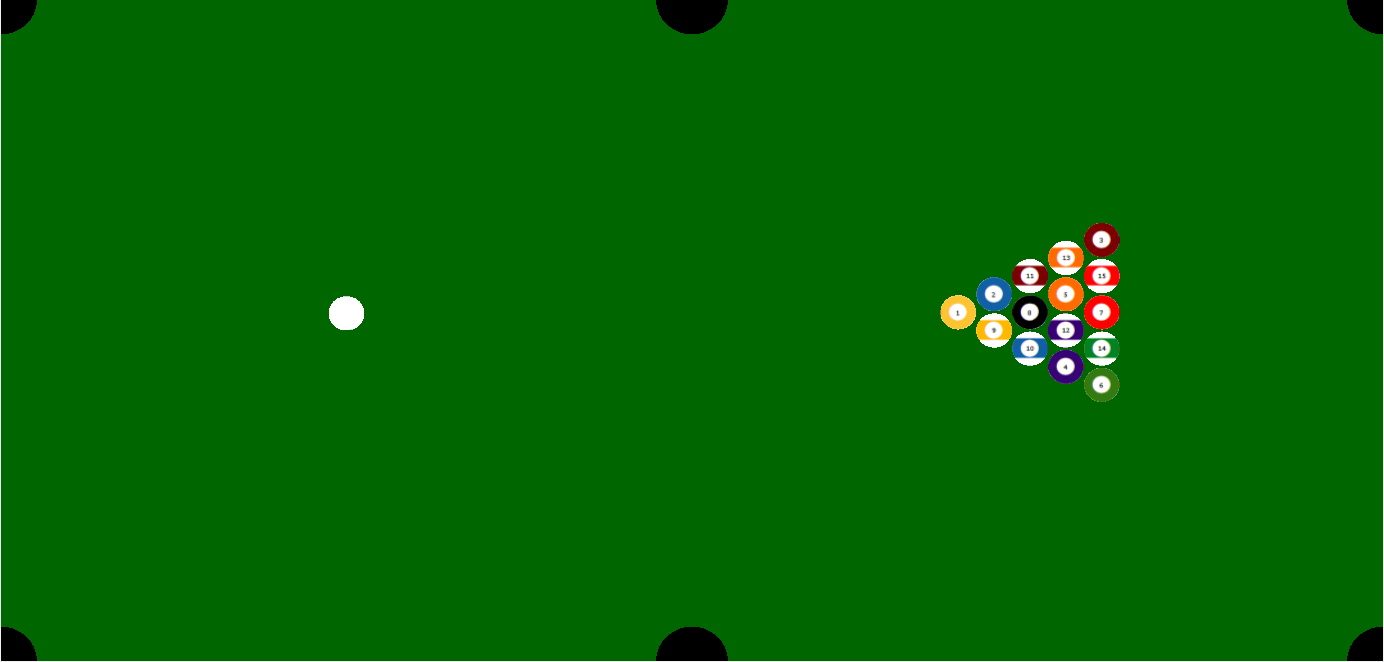
\includegraphics[width=\textwidth]{bilder/Spielfeld.png}
		 \end{figure}

